\subsection{過剰ノイズ}
増幅層がある半導体検出器特有のノイズとして、過剰ノイズ$\sigma_m$(Multiplication Noise)がある。
過剰ノイズは、電子雪崩によって生成される電子や正孔による、電流変化に起因するノイズである。
増幅層がある半導体内の単位長さあたりの電流変化は 式\ref{eq:current_Multiplication_Noise} のように表すことができる\cite{1363388845924852224}。
$\alpha$が電子のイオン化係数、$\beta$が正孔のイオン化係数として、
$\alpha I_n$は、電子が格子に衝突した時の単位長さあたりの電子正孔対の生成確率で、$\beta I_p$が、正孔が格子に衝突した時の単位長さあたりの電子正孔対の生成確率である。
$g$は、単位長さあたりの熱や光学的に生成される電子正孔対の生成確率である。
\begin{equation}
    dI_p=(\alpha I_n + \beta I_p + g)\:dx
    \label{eq:current_Multiplication_Noise}
\end{equation}
また、過剰ノイズ係数$\phi/{2eI_{\rm{{in}}}}$は 式\ref{eq:Multiplication_Noise} で表すことができる\cite{1363388845924852224}。
$\phi$は、過剰ノイズ分布密度である。また、$k=\frac{\beta}{\alpha}$で、$M$は増幅率である。
式\ref{eq:Multiplication_Noise} は注入電流$I_{\rm{{in}}}$が$I_p$で近似した場合に満たされる式となっている。
\begin{equation}
    \phi/{2eI_{\rm{in}}}=M^3 \left[1+\frac{1-k}{k}\left(\frac{M-1}{M}\right)^2 \right]
    \label{eq:Multiplication_Noise}
\end{equation}
式\ref{eq:Multiplication_Noise} を用いて、さまざまな$k=\frac{\beta}{\alpha}$での過剰ノイズ係数の増幅率依存性を 図\ref{fg:Multiplication_Noise} で示すことができる。
図\ref{fg:Multiplication_Noise} の縦軸が過剰ノイズ係数で横軸が増幅率の両対数グラフである。
このグラフを見ると、増幅率が高くなると過剰ノイズも大きくなることがわかる。そのため、増幅率が大きい領域では、過剰ノイズ増加により時間分解能が悪くなると考える。
また、$k=\frac{\beta}{\alpha}$の値によって過剰ノイズが変化することがわかる。
電子雪崩によって生成する電子と正孔の割合に偏りがあると、過剰ノイズの大きさに変化が生じる。
電子が高電場領域に入った時に電子の生成が多い場合と、正孔が高電場領域に入った時に正孔の生成が多い場合に、過剰ノイズが小さくなる。

LGAD検出器の時間分解能は増幅率の増加に従って信号のサイズが大きくなるため、式\ref{eq_TimingResolution} より導出される時間分解能は良くなるが、増幅層にかかる電圧をあげると過剰ノイズが増加する。
つまり、時間分解能の性能が最大になる最適な印加電圧が存在する。この電圧に関しては、4.4 章で詳しく述べる。通常、過剰ノイズが支配的になる領域より十分低い電圧での運転を行う。


\begin{figure}[h]
    \centering
    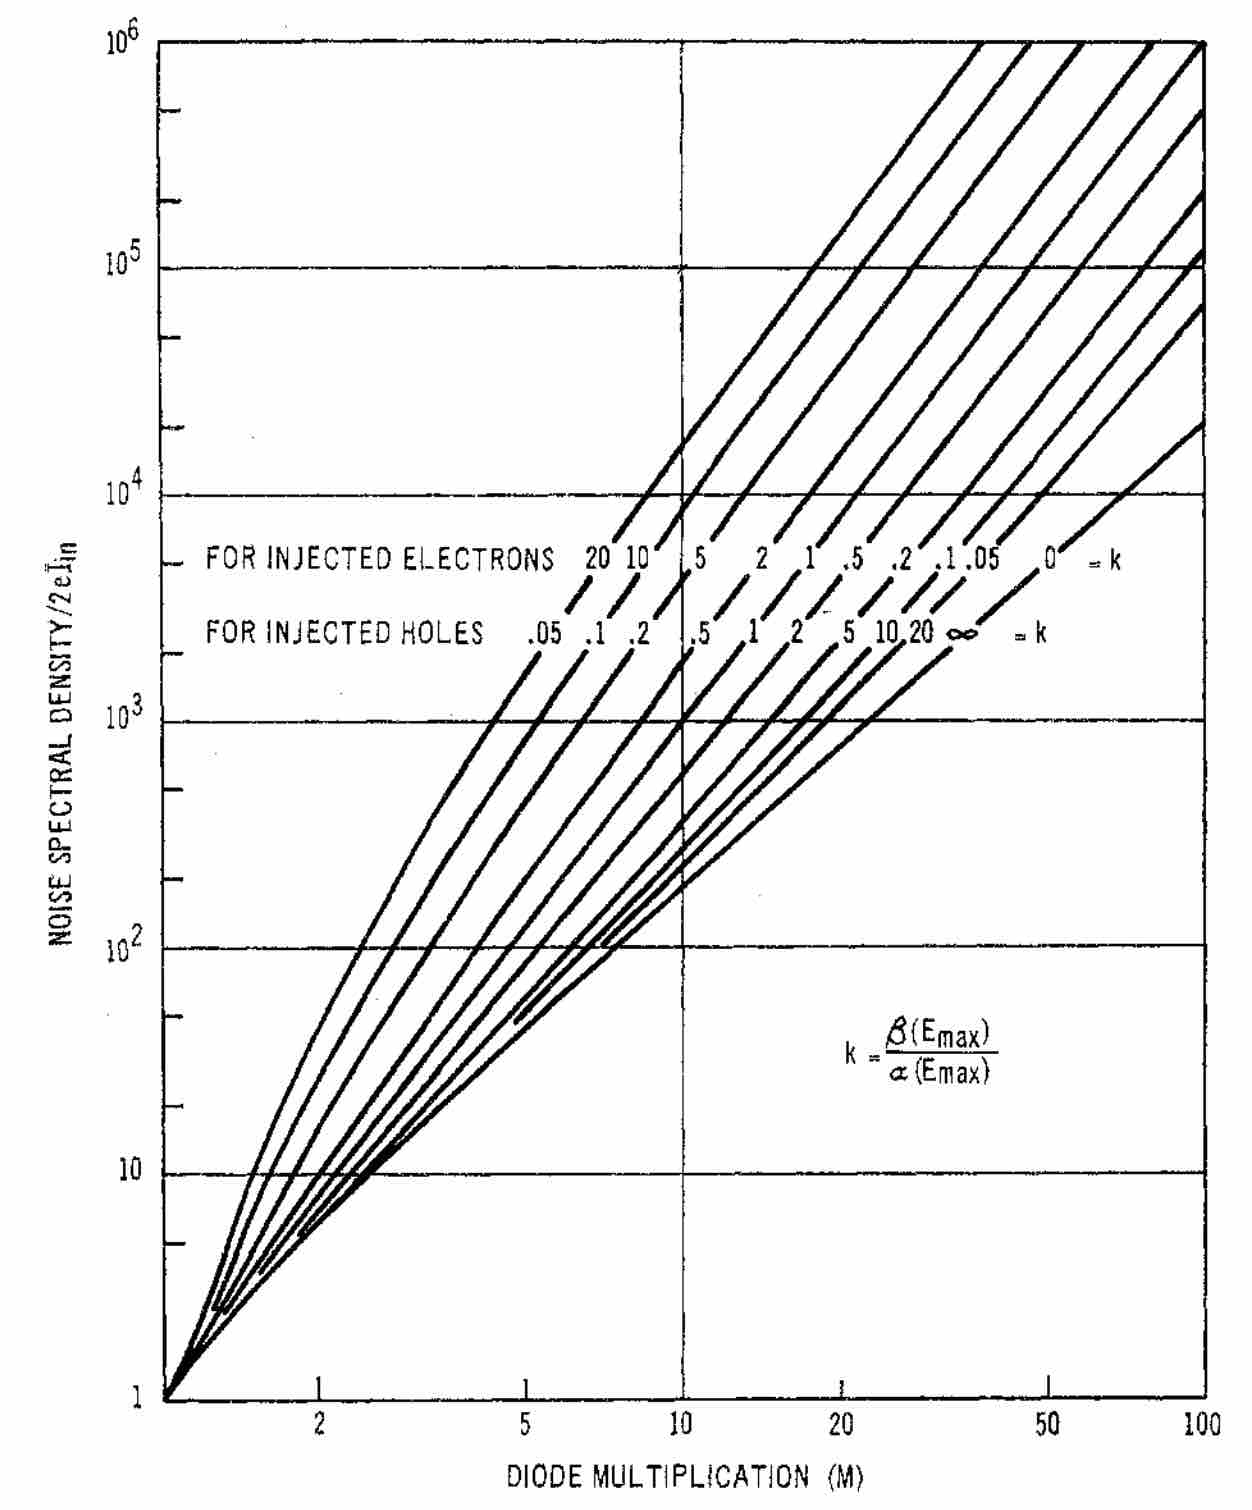
\includegraphics[width=7cm]{fig/ch3/Multiplication_Noise.jpg}
    \caption[過剰ノイズ係数の増幅率依存性\cite{1363388845924852224}]{過剰ノイズ係数の増幅率依存性\cite{1363388845924852224}\\横軸が増幅率で縦軸が過剰ノイズ係数の両対数グラフ、さまざまな$k=\frac{\beta}{\alpha}$での過剰ノイズ係数が示されている。}
    \label{fg:Multiplication_Noise}
\end{figure}

